\documentclass[a4paper]{scrartcl}
\usepackage{amsmath,amssymb,amsthm}
\usepackage{bm}
\usepackage{biblatex}
\usepackage{float}
\usepackage[colorlinks=true, allcolors = black, urlcolor=cyan]{hyperref}
\usepackage{graphicx}
\usepackage{mathtools}
\usepackage{physics}

\renewcommand{\thesection}{\arabic{section}}
\renewcommand{\thesubsection}{\alph{subsection}}

\title{Assignment 2}
\subtitle{TTK4210 - Advanced Control of Industrial Processes}
\author{Sondre Myrberg}
\date{\today}

\setlength{\parindent}{0pt} % Disable indentation
\mathtoolsset{showonlyrefs} % Only show equation numbers on referenced equations


\begin{document}

\hypersetup{pageanchor=false}
\begin{titlepage}
    \maketitle
    \vfill
    \vfill
    \vfill
    \vfill
    \vfill
    
\includegraphics[width=0.95\textwidth]{../ntnu_logo.pdf}
    \vfill
    \vfill
\end{titlepage}
\hypersetup{pageanchor=true}

\section{Model implementation}
The model given by
\begin{equation}
	\begin{aligned}
		G &= \left[
		\begin{array}{c|c}
			A & B \\
			\hline
			C & \bm{0}
		\end{array}
		\right]
		\\
		G_d &= \left[
		\begin{array}{c|c}
			A & B_d \\
			\hline
			C & \bm{0}
		\end{array}
		\right]
	\end{aligned}
\end{equation}
with $A$, $B$, $C$ and $B_d$ given in the exercise text is implemented as shown in \autoref{fig:1model}.
\begin{figure}[ht!]
	\centering
	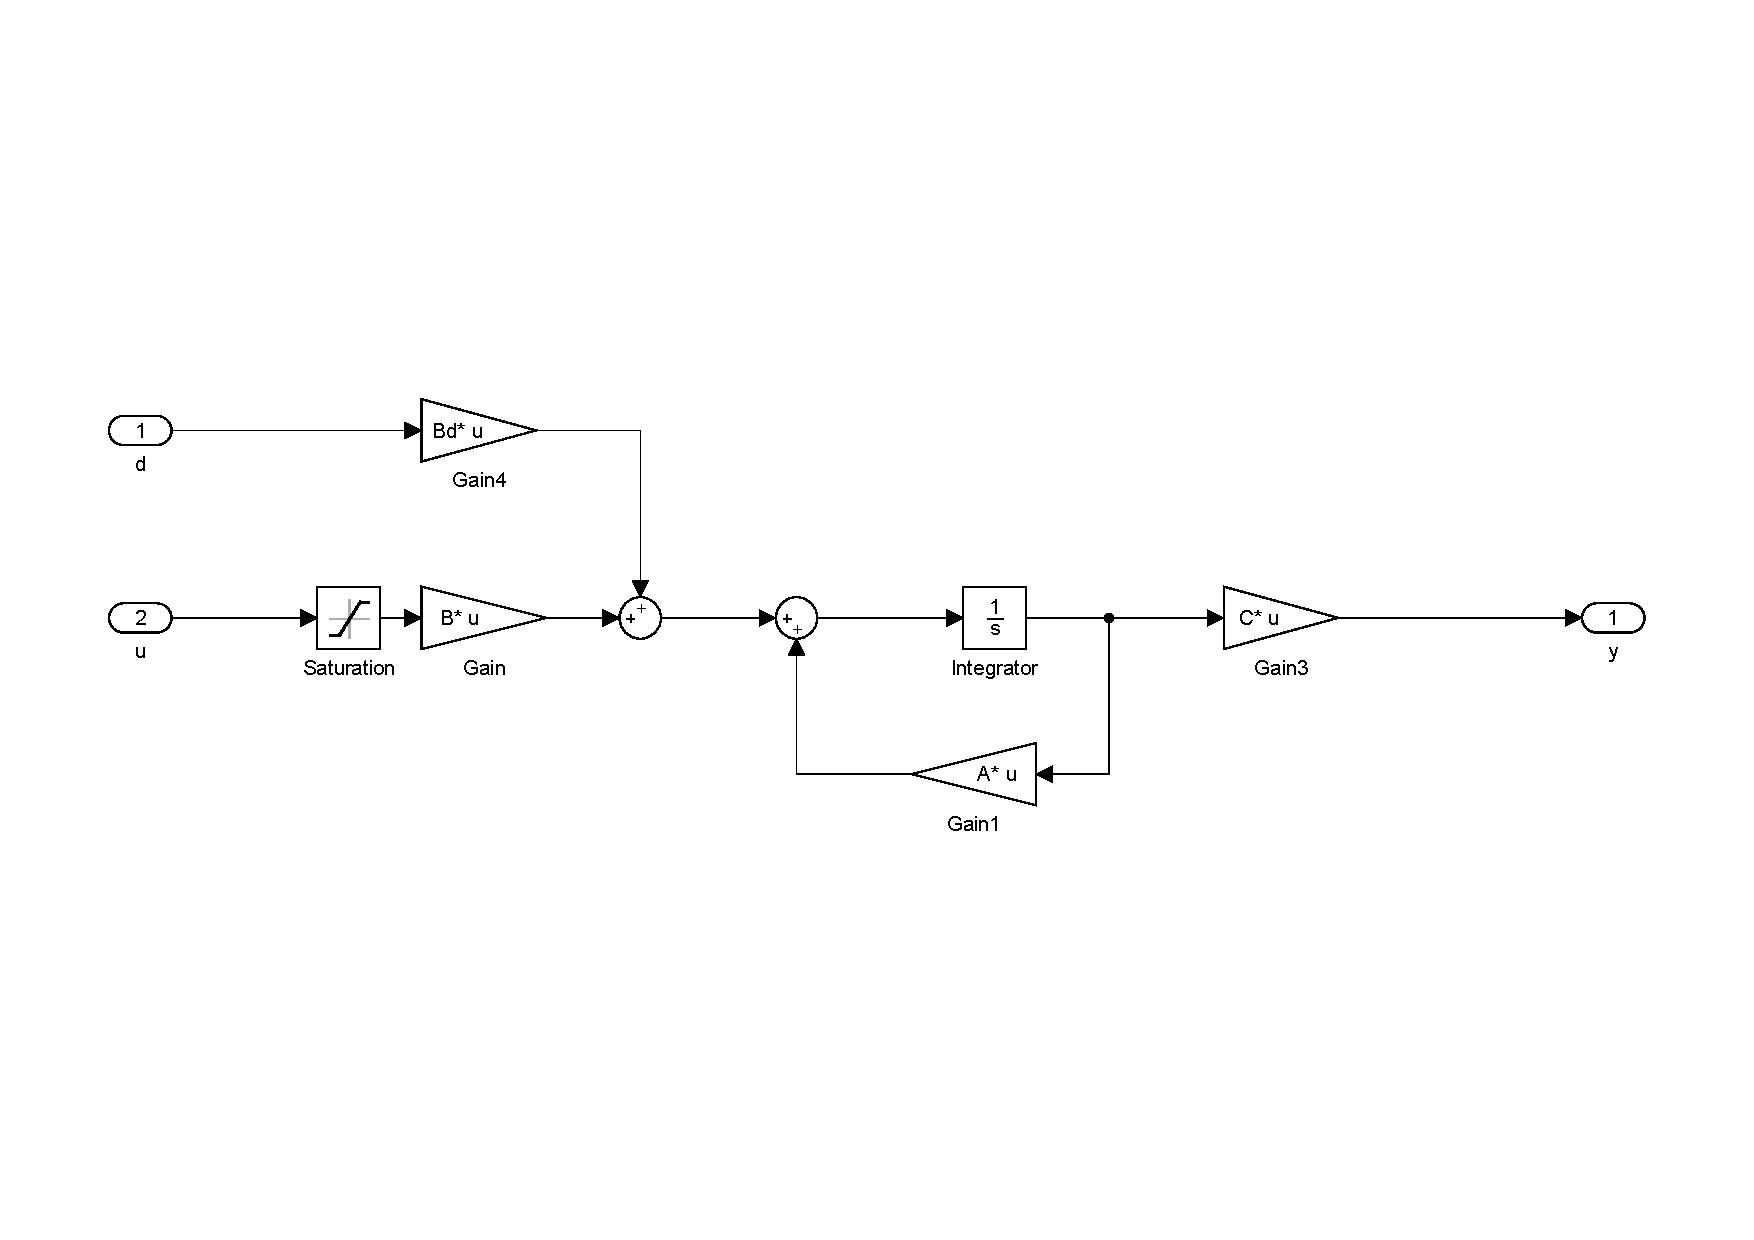
\includegraphics[width=0.8\textwidth]{fig/LV.pdf}
	\caption{Simulink model of LV-model}
	\label{fig:1model}
\end{figure}

\end{document}